%%%%%%%%%%%%%%%%%%%%%%%%%%%%%%%%%%%%
\chapter{Introduction}
\label{chap:Introduction}
%%%%%%%%%%%%%%%%%%%%%%%%%%%%%%%%%%%%

\comment{

The introduction should provide:
\begin{itemize}
    \item A clear explanation of the problem that you tackle
    \item Motivation why this is interesting and worth investigating
\end{itemize}

To improve communication, it is also recommended that you concisely state the aims and objectives of your project.  As part of the introduction, these can be generally stated and not require specialist knowledge.  Use the next chapter "Literature Review" to provide specialist knowledge for the reader.
\begin{enumerate}
    \item \textbf{Aims:} The aims of a project are \emph{what you hope to learn}.
        \begin{enumerate}
        \item "To understand why X varies with Y..."
        \item "To evaluate [technology] when exposed to unexpected conditions so that..."
        \item "To increase understanding of ..."
        \item \emph{etc...}
        \end{enumerate}
    \item \textbf{Objectives:} The objectives are \emph{the elements which are necessary to conduct the project}.
        \begin{enumerate}
            \item "To properly design an experiment methodology to mitigate...."
            \item "To construct a robotic system including ... to collect meaningful data."
            \item "A complete analysis of ... must be conducted prior to the full system evaluation in order to..."
            \item \emph{etc...}
        \end{enumerate}
\end{enumerate}

You can then repeat and address these explicitly in your Conclusion when evaluating the success and challenges of your project. 
    
}

\section{Brief Introduction}
\label{chap:Brief Introduction}
% 本项目的主旨是尝试将一种用于通讯的时分复用技术的思想用于多机器人之间的去中心化无碰撞路径生成中
The main idea of this project is to attempt to utilise the principles of a decentralised channel sharing communication protocol (\textit{Self-organised Time Division Multiple Access}, STDMA\cite{STDMA}) to achieve collision-free movement among multiple decentralised agents on a 2D plane.

\subsection{Principles of STDMA}


% STDMA允许agent在信道中实现无冲突的时分复用。即,在每一时刻只有一个agent发送信息,且在正常情况下此信息不会和其他agent碰撞(即,不会有多个agent选择在同一时刻发送信息)。
In STDMA, a 1D channel is represented with repeating frames that are consisted of discrete time slots.

STDMA enables agents to achieve \textbf{S}elf-organised \textbf{T}ime-\textbf{D}ivided \textbf{M}ulti-\textbf{A}ccess within the channel. That is, each agent independently finds a slot which is uniquely its own and uses this slot to broadcast its message.

\textbf{The key idea of STDMA} is to determine empty slots and apply for them.

This idea also works for collision-free moving on 2D plane —— to determine free space and apply for usage.

For detailed explanation about STDMA, please see \textbf{PLACEHOLDER}.

\subsection{The 2D Plane}

The 2D plane used in this project is represented with discrete pixels / grids, just like the STDMA protocol represents continuous time with discrete slots.

For such a representation of a 2D plane, there is a term called \textbf{grid world}\cite{GridWorld}.

For detailed assumptions, please see \textbf{PLACEHOLDER}.

\subsection{Agents}

To meet the requirement of decentralisation, the agents are assumed to be identical.

The agents can:
\begin{itemize}
    \item Broadcast and receive messages in the given channel, but cannot do both at the same time (i.e., cannot be listening while speaking or speaking while listening).
    \item Move only one step / one grid in the map in one time step.
\end{itemize}

For detailed assumptions, please see \textbf{PLACEHOLDER}.


\section{Aims}
\begin{itemize}
    \item Based on the idea of STDMA, design an algorithm for decentralised agents to achieve colission-free movement and space sharing on 2D plane.
    \item Evaluate the advantages and drawbacks of the designed algorithm, and therefore get a better understanding on the problem that the alrogithm aims to solve.
\end{itemize}
\section{Objectives}
\begin{enumerate}
    \item Implement original STDMA communication protocol with ROS2, use nodes in ROS2 as agents in the channel, achieve self-organised channel sharing and communicating among agents.
    \item Design the specific algorithmic content for agents to achieve collision-free movement.
    \item Implement the designed algorithm with ROS2, use ROS2 nodes as agents moving on the 2D plane.
    \item Build proper test scene and performance evaluator that could extract metrics (makespan, average finish time, etc.) from simulations.
    \item Examine the advantages, disadvantages and limitations of the designed algorithm, summarize the results from observations.
\end{enumerate}

\section{Motivation}

The motivation of this project is to answer a question which is inspired by \cite{Paper_From_Supervisor}, which is:

\begin{quote}
    \textbf{What would happen if use STDMA for dencentralised 2D resource sharing and path planning?}
\end{quote}

And this quesiton could be seperated to the following two parts:

\subsection{Why STDMA?}

The reason for using STDMA is its \textbf{characteristics}\cite{STDMA_characteristic}:

\begin{enumerate}
    \item \textbf{Deterministic}: Agents arrange their data transmission based on a determined timetable.
    \item \textbf{Decentralised}: Agents listen to the channel first, then independently seek and allocate free slots for themselves to use.
\end{enumerate}

These characteristics are useful for multiple agents to achieve collision-free (use free slots only), slf-organised (find slots on its own) moving and resource sharing.

There are also \textbf{reasons that making this challenging}:
\begin{enumerate}
    \item \textbf{Dimensional Difference}: STDMA is designed for sharing discrete time slots (1D), and cannot be directly applied for resource sharing on a 2D plane. Modification is needed for 2D application.
    \item \textbf{Moving by Grids}: In the communication scenario, agents don't have destiniations in the timetable, i.e., don't need to move to specific slot in the timetable. But that's different for 2D space moving, where agents have their destinations and need to move grid by grid to reach their goals. Agents could easily be trapped in situations of inefficiency or even deadlock situations \cite{MAPF_Deadlock_Explain1,MAPF_Deadlock_Explain2}.   
\end{enumerate}

These characteristics and challenges are making this topic interesting and worthy for investigation.

\subsection{Why decentralised 2D resource sharing and path planning?}

There are many algorithms aim to solve this problem, and their shared aspect is a \textbf{focus on the movement of multiple decentralised agents within a grid world}. 

To easily get a better understanding of this problem, please refer to this \href{https://primalgrid.netlify.app/primal}{website}\footnotemark.\footnotetext{https://primalgrid.netlify.app/primal} 
This website presents the problem scenarios and their solutions through a simple and engaging animation (estimated time required: 1$\sim$2 min). 
For detailed explanation, please see \textbf{PLACEHOLDER}.

For such situations, \textbf{there are myriad corresponding real-life problems and applications}.

\begin{figure}
    \centering
    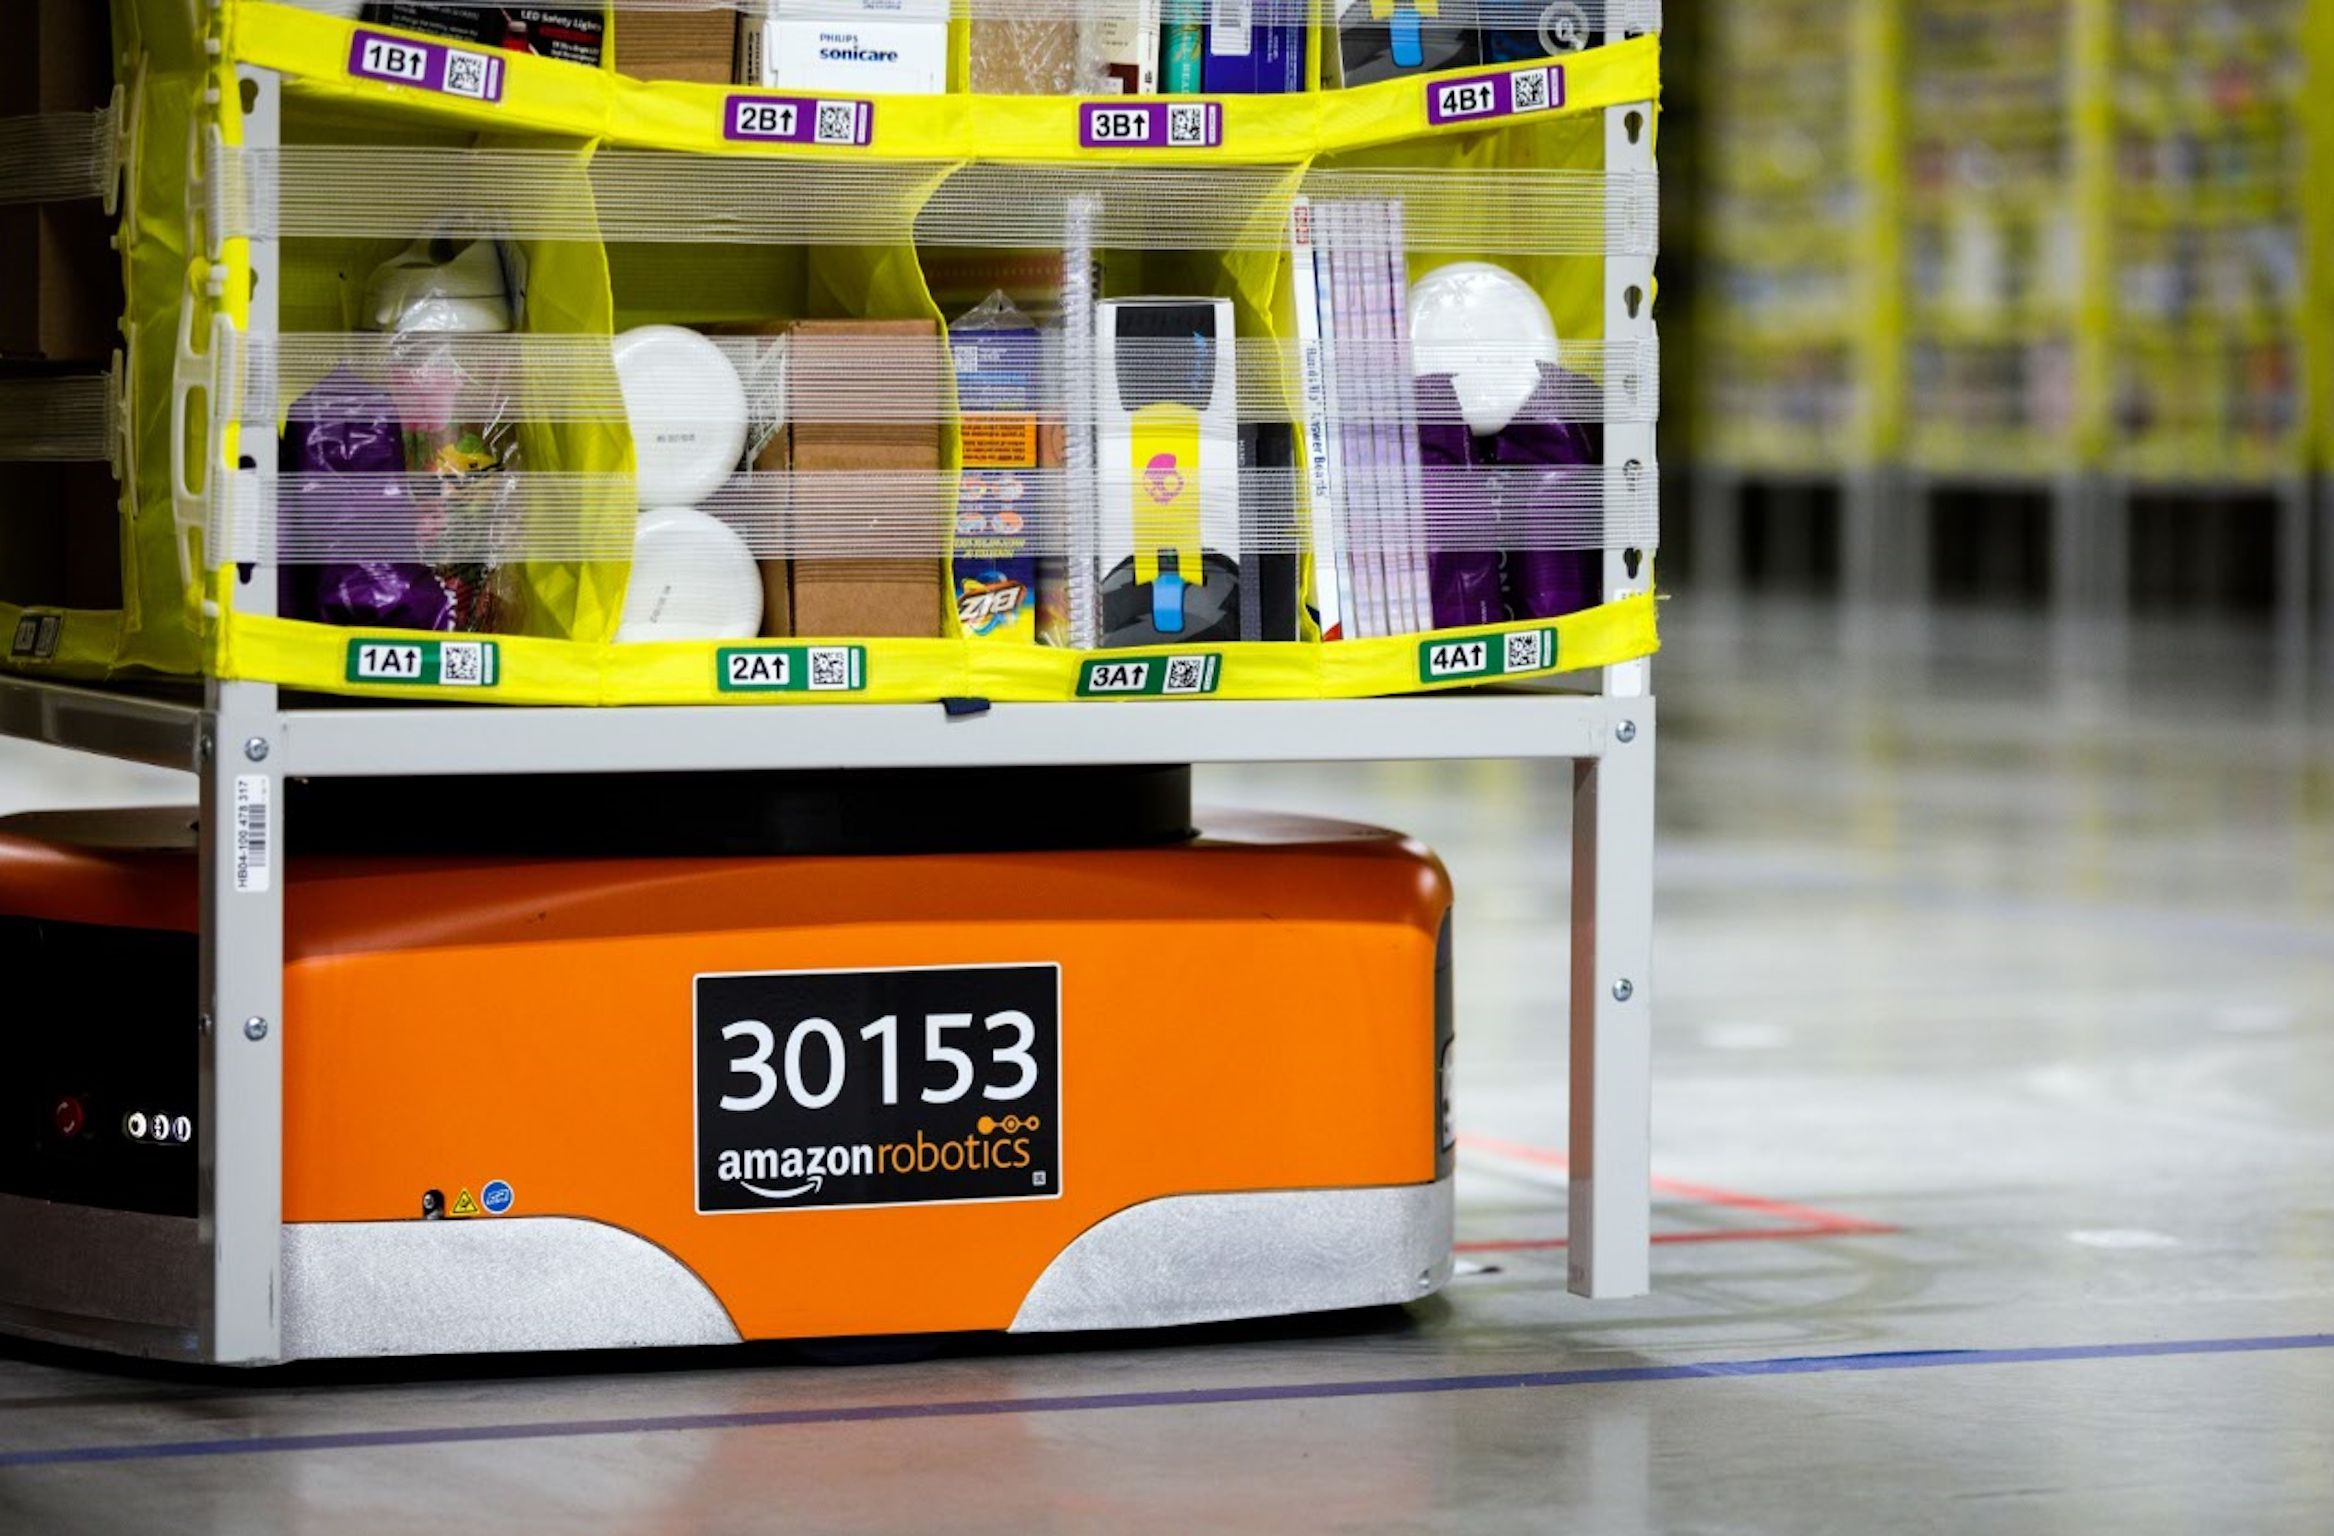
\includegraphics[width=0.6\linewidth]{figures/Amazon_Warehouse.jpeg}
    \caption{Kiva system operating in Amazon warehouse.\protect\footnotemark}
    \label{fig:Amazon Warehouse Robots}
\end{figure}

\footnotetext{https://spectrum.ieee.org/interview-brad-porter-vp-of-robotics-at-amazon}


\begin{itemize}
    \item \textbf{Warehouse Automation}: Automated pick-pack-and-ship system in warehouse (like Fig \ref{fig:Amazon Warehouse Robots}.) \cite{Amazon_Kiva}. Delivering items in sorting station\cite{Warehouse_Automation1,Warehouse_Automation2}.
    \item \textbf{Intersection Management}: Coordinate autonomous vehicle movement through intersections \cite{Intersection_Management}.
    \item \textbf{Robot Fleet}: Automating fleets of autonomous robots like forklift fleets \cite{Fork_Fleet1,Fork_Fleet2}.  
    \item \textbf{Agents in video games and CGIs}: Flock simulating and animating\cite{Flocking_1,Flocking_2}.
    \item \textbf{Swarm Robots}: Controlling self-organised robot swarms\cite{Swarm_Robotics}.
\end{itemize}

In general, the application of this algorithm is very broad. Furthermore, in the context of Industry 4.0 and flexible manufacturing, it has even better prospects for application\cite{Industry_41,Industry_42,Industry_43}, as centralized control is gradually becoming inadequate to meet new production needs.
